% Exmaple thesis using jthesis class
% Written by George Taylor (gstaylor@iee.org)
%
% Please mail all comments and changes to G.S.Taylor@ee.ed.ac.uk
% so that this package can be kept up to date.

\typeout{PhD Thesis class example}

% Supported options to jthesis:
%	nohyphens 		make hyphenation incredibly unlikely
%				(the university guidelines suggest this)
%				if you get an awakward line you will need
%				to either change it, or use \-
%
%	doublespace		double space eveything except
%				contents, lists of figures etc and references
%				Personally I think double spacing sucks.
%				Use \begin,end{singlespace} for exceptions.
%				(safe to use even when doublespace option
%				 not given)
%
% Other options (not part of jthesis) which you may wish to use:
% twoside - for two sided output
% fleqn - left indented (rather than centered) equations
%
\documentclass[doublespace]{StyleFiles/jthesis-v1}

% By default a eps file of the University Crest is assumed to be
% in the StyleFiles directory. However you may wish to give a full
% absolute pathname here so that xdvi, dvips etc work even when run
% from another directory.
%\crestfile{/home/gst/PhD/Thesis/StyleFiles/EdUniCrest.eps}

% The array package extends tabular, for example useful for <{$},>{$}
% when using tables of symbols
\usepackage{natbib}
\usepackage{array}

% It is recommended you use amsmath for better looking equations,
% but the jthesis class does not enforce this.
\usepackage{amsmath}

% Use subfigure to put multiple figures into one - complete with
% mini captions.
%\usepackage{subfigure}
\usepackage{subfig}

% Other useful packages you might not otherwise find out about:

\usepackage{booktabs}
% \usepackage{psfrag}	% replace labels in xfig diagrams with nice math
% \usepackage{endfloat} % put all floats at end
% \usepackage{shadow}   % for shadowed boxed round things
% \usepackage{bar}	% for bar charts
% \usepackage{draftcopy} % prints DRAFT across each page in big grey letters
% \usepackage{mathtime}  % for times font style maths (may require some fonts)
% see also the documentation for the graphicx package providing
% support for postscript images and colour (already \usepackage'd)

\usepackage{dcolumn}
\usepackage{hyperref}
\usepackage{tabularx}
\usepackage{lscape}
\usepackage{graphicx}
\usepackage{rotating}

% Tip: If you include your own .sty/.cls files with \usepackage
% instead of \include separate .aux files will not be generated for
% each included file.
%\usepackage{StyleFiles/mymacros}


% Tip: use \includeonly to only include one thing and ignore all other
% \include commands, this is handy for formatting only one chapter
% at a time
%\includeonly{Chapter1/chapter1}


\begin{document}

% Put your title, your name, and submission date here
% use \date{} if you don't want a date, todays date is used
% if \date is omitted.
\title{My Very interesting Thesis}
\author{Sam Hawkins}
\date{September 2010}

\maketitle

% If you look in the included files you will notice the use of
% \minorchapter.

\include{Preliminary/abstract}
\include{Preliminary/declaration}
\include{Preliminary/acknowledgements}

% Insert table of contents and lists of figures and tables.
\contentsandlists

% More use of minorchapter
\include{Preliminary/abbreviations}
\include{Preliminary/nomenclature}

% \startchapters indicates the main chapters follow, this changes
% things such as the page numbering.
\startchapters

\chapter{Introduction}

This is the beginning. I bet you wish that you had very started before long. I
shall now write two paragraphs. This is the second paragraph. In recent times
the way in which the human race uses and generates its energy has become of
extreme social, economical and environmental importance. Predictions of damaging
increases in mean global temperatures \citep[see][]{Solomon:2007:CUP} has
increased the need for carbon emitting energy technologies to be replaced by low
carbon alternatives. Additional long term economic factors are also playing
their part in shifting momentum to new technologies, in particular the concerns
about oil and natural gas supplies. Demand for oil and gas is expected to
outstrip supply within the current century, leading to inflated prices and
energy security issues. Unfortunately, although the resource and environmental
issues are occurring simultaneously, they are not necessarily mutually
supportive. For instance, once the price for oil has reached a certain value it
can be economically synthesised from coal, providing no environmental benefits.
In fact, if the market were left to choose a method for replacing dwindling oil
resource then this is one of the most likely substitutes; even in light of
population growth, coal reserves are estimated to last for hundreds of years
\citep[see][]{Jaccard:2005:CUP} and thus the cost is low.

With markets failing to deliver the necessary changes, it has become the
responsibility of governments to intervene under the premise that the predicted
environment and economical consequences of inaction will outweigh the costs
incurred by immediate action. This is a tough political task as, particularly in
the UK, energy markets have followed a trend of liberalised trading which makes
strategic decision making extremely challenging. Private investment is unlikely
to match policy, unless the policy is seen to be long term and economically
advantageous; a virtual impossibility when scientific and economic opinions of
the market requirements are so uncertain. In addition, the likelihood of direct
governmental intervention in the form of capital investment is now looking more
unlikely, due to the recent financial crisis. Capital spending is set to fall
significantly in order to reduce deficits endured to rescue the banking sector.

Despite the potential funding problems, the United Kingdom (UK) Government's
Climate Change Act 2008 \citep*[see][2008]{CCA:2008:Defra} introduced for the
first time legally binding targets for greenhouse gas emissions from within the
UK. The targets set an 80\% reduction of greenhouses gases by 2050 and a 26\%
reduction of carbon-dioxide $\text{CO}_{2}$ emissions by 2020 with respect to
1990 levels. This is set in the context of Britain's pre-existing target to
reduce emissions by 12\% as a ratified signatory of the Kyoto Protocol
and a European Union proposal to cut EU wide greenhouse gas emissions by 20\% by
2020 each with respect to 1990 levels. Electricity generation in the United
Kingdom accounts for 37\% of all emissions and as part of the
government's greenhouse gas reduction strategy it will seek to reduce this to
zero by 2030 \citep[see][2008]{CCC:2008}. Given the enormity of this task it is
foreseen that a varied mix of low/zero carbon electricity generating
technologies will be required.
\begin{quote}
 ``It is a well known fact that the use of a high-order panel method is more
accurate than the
low-order panel method or the discrete vortex method in computing the velocity
field as the
appearance of instabilities in the vortex sheet due to the spurious numerical
effects introduced by
a too-crude representation.''
\end{quote}
As such, a melting pot of renewable and sustainable energy technologies have
begun to compete to become part of a `post-carbon' energy mix. Some of these
technologies are well established, such a nuclear, biomass and wind, others less
so, such as solar photovoltaic and marine energy. In addition, carbon emitting
technologies such as coal remain an attractive option for governments and
investors alike, as carbon capture and storage technology promises to store away
the greenhouse gases emitted in combustion. However, carbon capture and storage
is still an unproven technology and thus, the future costs of this and many
other of the new energy technologies are hard to predict and are, at present,
highly contestable; ultimately, over the long term, energy cost is the most
likely deciding factor as to which technologies will feature most. Hence, each
industry is working hard to reduce costs via research and innovation.

\chapter{Another Chapter}

\section{The first section}

Note that all section and chapter titles should use lower case except
for the first character of the first word. Here is a reference to a
paper~\cite{apaper}. Figure~\ref{fig:picture} is a weird picture.

\begin{figure}[h]
  \centering
  %% Because graphicspath was set in edengths.tex you only need to
  %% supply the file name here, i.e. examplepicture (doesn't need the
  %% extension) and not the full path. Just remember to add the path
  %% to \graphicspath{{thispath/}{thatpath/}}
  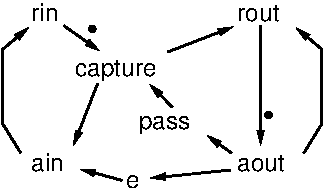
\includegraphics[width=2in]{examplepicture}
  \caption[Long caption and \textit{some italics} to see what happens]%
  {This is an example of pdf with a very long caption and \textit{some italics} to see what happens and it should see what happens over two lines.}
\label{fig:picture}
\end{figure}

\subsection{A subsection}

Lorem ipsum dolor sit amet, consectetur adipiscing elit. Maecenas nec orci lacus, ac sollicitudin tortor. Maecenas rutrum vestibulum rhoncus. Vestibulum non ligula nibh. Cum sociis natoque penatibus et magnis dis parturient montes, nascetur ridiculus mus. Phasellus egestas sodales lacus, ac scelerisque nulla venenatis sed. Ut elementum turpis ac lacus consectetur consequat. Sed at est eros. Praesent erat velit, dictum id adipiscing eu, ultrices vel nisi. Nullam at nisl ut est posuere commodo tincidunt eget nisl. Integer id erat non metus adipiscing dignissim quis sed enim. Curabitur viverra lobortis eleifend. Proin vestibulum nunc eu augue dapibus quis porttitor ipsum rhoncus. Duis tortor tellus, suscipit sit amet ornare id, lacinia sed lacus. Ut in molestie ligula. Praesent euismod lectus vitae arcu malesuada tempus. Aliquam pharetra tincidunt augue in eleifend. Curabitur porttitor vulputate quam, ut fringilla mauris porta eu. Curabitur sodales, felis non vestibulum feugiat, urna diam bibendum purus, ac scelerisque massa eros sit amet ipsum. In elementum laoreet aliquam.

\subsubsection{A subsubsection}

Aliquam eget sapien tellus, sed rutrum leo. Vestibulum et quam sit amet dolor gravida sagittis. Aenean dapibus urna a nibh sollicitudin pharetra. Sed nisi augue, vehicula sed tristique facilisis, lacinia ut augue. Nam quis tempor mi. Vestibulum lorem leo, aliquet at sollicitudin vitae, fringilla id odio. Aenean a orci odio. Mauris tincidunt eros ac libero suscipit molestie. Donec feugiat turpis a urna suscipit in pellentesque magna pretium. Vivamus eget nunc vitae nunc ultricies tincidunt. Duis dictum eros et lorem auctor id ullamcorper diam commodo. Pellentesque quis dolor nec urna vestibulum pellentesque. Donec luctus mi ut nisi hendrerit pulvinar. Donec fringilla, lectus vitae accumsan sollicitudin, sem metus mollis risus, nec laoreet ante arcu ut augue.

\subsection{Another subsection}

Table~\ref{tab:atable} is an example of a~\footnote{this is a
footnote} simple table.

\begin{table}[htb]
\begin{center}
\begin{tabular}{|c|c|c|}
\hline
1.0 & 2.0 & 3.0 \\
\hline
4.0 & 5.0 & 6.0 \\
\hline
\end{tabular}
\caption{A table}
\label{tab:atable}
\end{center}
\end{table}


\section{Another section}

This is a long and boring paragraph for the purpose of testing the
spacing between paragraphs and the use or otherwise of indentation. I
think a space between paragraphs and without the first line indented
is somewhat easier to read than no space between paragraphs and with
the first line indented.

Another equally exciting paragraph, one two three four five six seven
eight nine ten eleven twelve thirteen fourteen fifteen sixteen
seventeen eighteen nineteen twenty and so on.

\begin{equation} \label{eqn:dct}
z(k,l) = \frac{2}{N} \alpha(k) \alpha(l) \sum_{m=0}^{N-1} \sum_{n=0}^{N-1}
         x(m,n) \cos \frac{ (2m+1) \pi k}{2N} \cos \frac{ (2n+1) \pi l}{2N}
\end{equation}

\begin{equation} \label{eqn:idct}
x(m,n) = \frac{2}{N} \sum_{k=0}^{N-1} \sum_{l=0}^{N-1}
         \alpha(k) \alpha(l) z(k,l)
\end{equation}

\begin{quotation}
This is a quotation, another equally exciting paragraph, one two three
four five six seven eight nine ten eleven twelve thirteen fourteen
fifteen sixteen seventeen eighteen nineteen twenty and so on. Just
checking it is single spaced.
\end{quotation}

\frontchapter{Nomenclature}

\section*{Main equations}
\begin{equation}
  a=\frac{N}{A}
\end{equation}%
\nomenclature{$a$}{The number of angels per unit area}%
\nomenclature{$N$}{The number of angels per needle point}%
\nomenclature{$A$}{The area of the needle point}%
The equation $\sigma = m a$%
\nomenclature{$\sigma$}{The total mass of angels per unit area}%
\nomenclature{$m$}{The mass of one angel}
follows easily.

\include{Chapter4/chapter4}
\include{Chapter5/chapter5}
\include{Chapter6/chapter6}


% \appendix indicates from now on \chapter generates an appendix
% rather than a normal chapter.
\appendix

%\include{Appendix/appendixA}

% \insertreferences inserts the list of references using the IEEE style
% and updates the table of contents. The single argument is a comma
% spearated list of .bib files (just as in \bibliography)
\insertreferences{References/library}

% that's all folks!
\end{document}








